%UNIT 1: QUALITATIVE AND GRAPHICAL APPROACHES
% Is 2nd part of original 01.tex
%%%%%%%%%%%%%%%%%%%%%%%%%%%
%%%% Put the following at the top of each .tex file  %
\pagestyle{fancy}
\renewcommand{\theUnit}{1.2}
\ifthenelse{\isundefined{\UnitPageNumbers}}{}{\setcounter{page}{1}}
\rhead{Section \theUnit: Slope Fields}
\lhead{
\includegraphics[width=1.25cm]{IODE-logo.png}}
\rfoot{\mypage}
\lfoot{}
\cfoot{}
\fancypagestyle{firstfooter}{\footskip = 50pt}
\renewcommand{\footrulewidth}{.4pt}
%%%%%%%%%%%%%%%%%%%%%%%%%%%
\vspace*{-20pt} \thispagestyle{firstfooter}
\pagebegin{Slope Fields}

A \textbf{slope field} is a graphical representation of a rate of change equation. Given a rate of change equation, if we plug in particular values of $(t,y)$ then $\displaystyle\frac{dy}{dt}$ tells you the slope of the tangent vector to the solution at that point.
\vs
For example, consider the rate of change equation $\displaystyle\frac{dy}{dt}=y+2t$.  At the point (1, 3), the value of $\displaystyle\frac{dy}{dt}$ is 5. Thus, the slope field for this equation would show a vector at the point (1, 3) with slope 5.  A slope field depicts the exact slope of many such vectors, where we take each vector to be uniform length. Slope fields are useful because they provide a graphical approach for obtaining qualitatively correct graphs of the functions that satisfy a differential equation.

\begin{enumerate}
\item Below is a partially completed slope field for  $\displaystyle \frac{dP}{dt}=0.8P$. \label{01problem7}
\begin{enumerate}
\item	Plot many more tangent vectors to create a slope field. \label{01problem7parta}
\item	Use your slope field to sketch in qualitatively correct graphs of the solution functions that start at $P = 0, 0.5$, and $2$, respectively. Note: the value of $P$ at an initial time (typically $t = 0$) is called an \textbf{initial condition}. \label{01problem7partb}
\item	Recall that a solution to a differential equation is a function that satisfies the differential equation. Explain how the graph with initial condition $P(0) = 1$ can graphically be thought of as a solution to the differential equation when the differential equation is represented by its slope field. \label{01problem7partc}
\end{enumerate}

\begin{center}
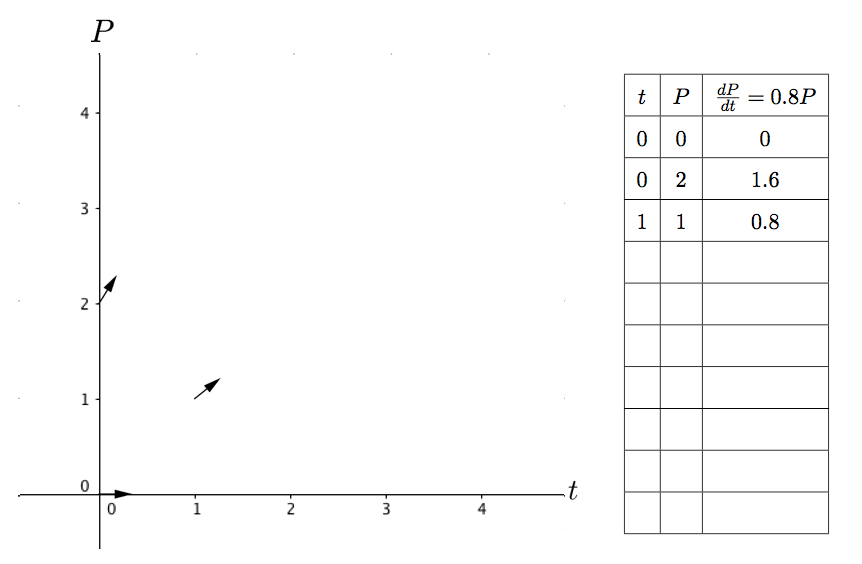
\includegraphics[width=6in]{02/02MyFirstSlopeFieldwithTable.png}
\end{center}

\clearpage

\item Below are seven rate of changes equations and three different slope fields. Without using technology, identify which differential equation is the best match for each slope field (thus you will have four rate of change equations left over). Explain your reasoning. \label{01problem8}
\[
\text{(i) } \frac{dy}{dt}=t-1 \quad \text{(ii) } \frac{dy}{dt}=1-y^2 \quad \text{(iii) } \frac{dy}{dt}=y^2-t^2 \quad \text{(iv) } \frac{dy}{dt}=1-y
\]
\[
\text{(v) } \frac{dy}{dt}=t^2-y^2 \quad \text{(vi) } \frac{dy}{dt}=1-t \quad \text{(vii) } \frac{dy}{dt}=9t^2-y^2
\]
\begin{enumerate*}
\item 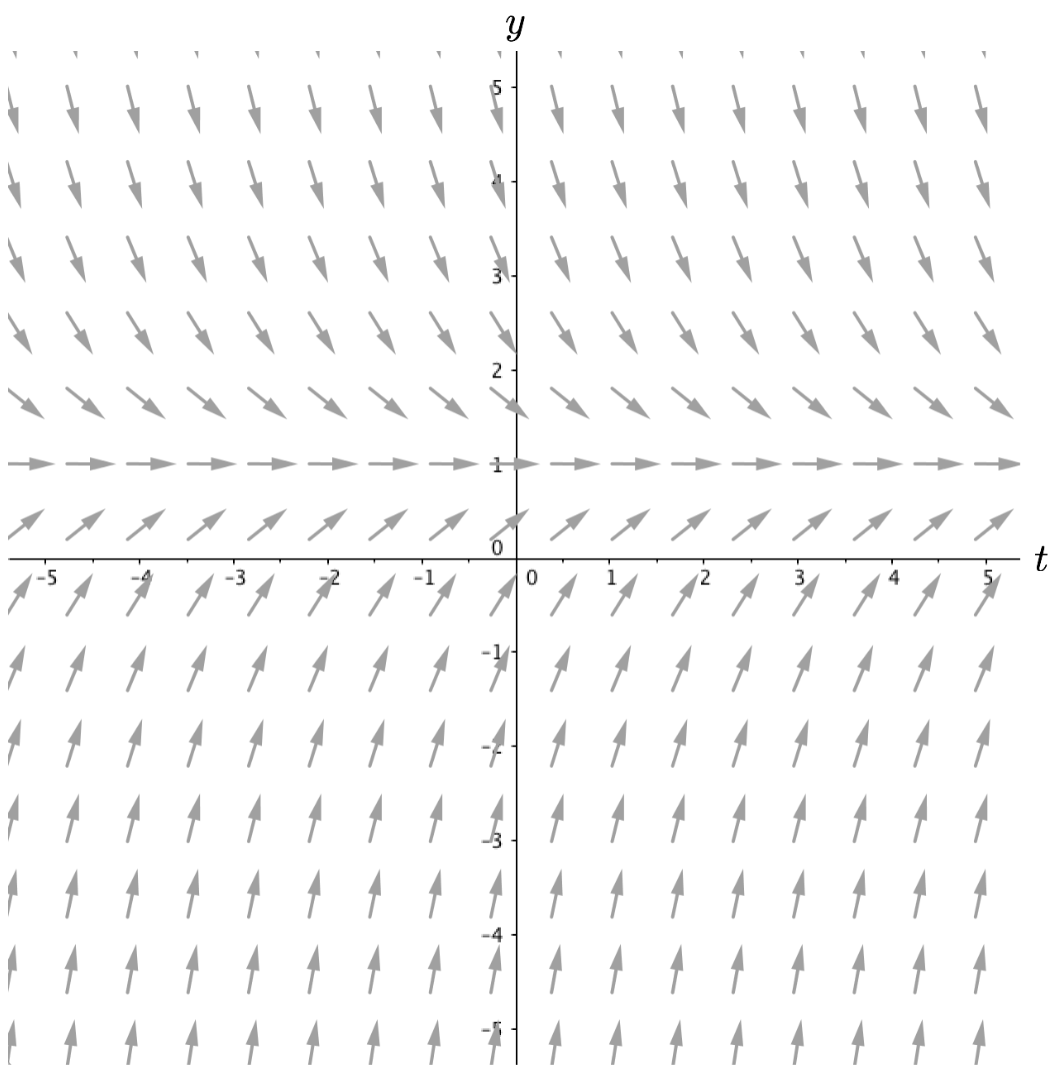
\includegraphics[width=2.75in]{02/02SlopeField1.png} \label{01problem8parta}
\item 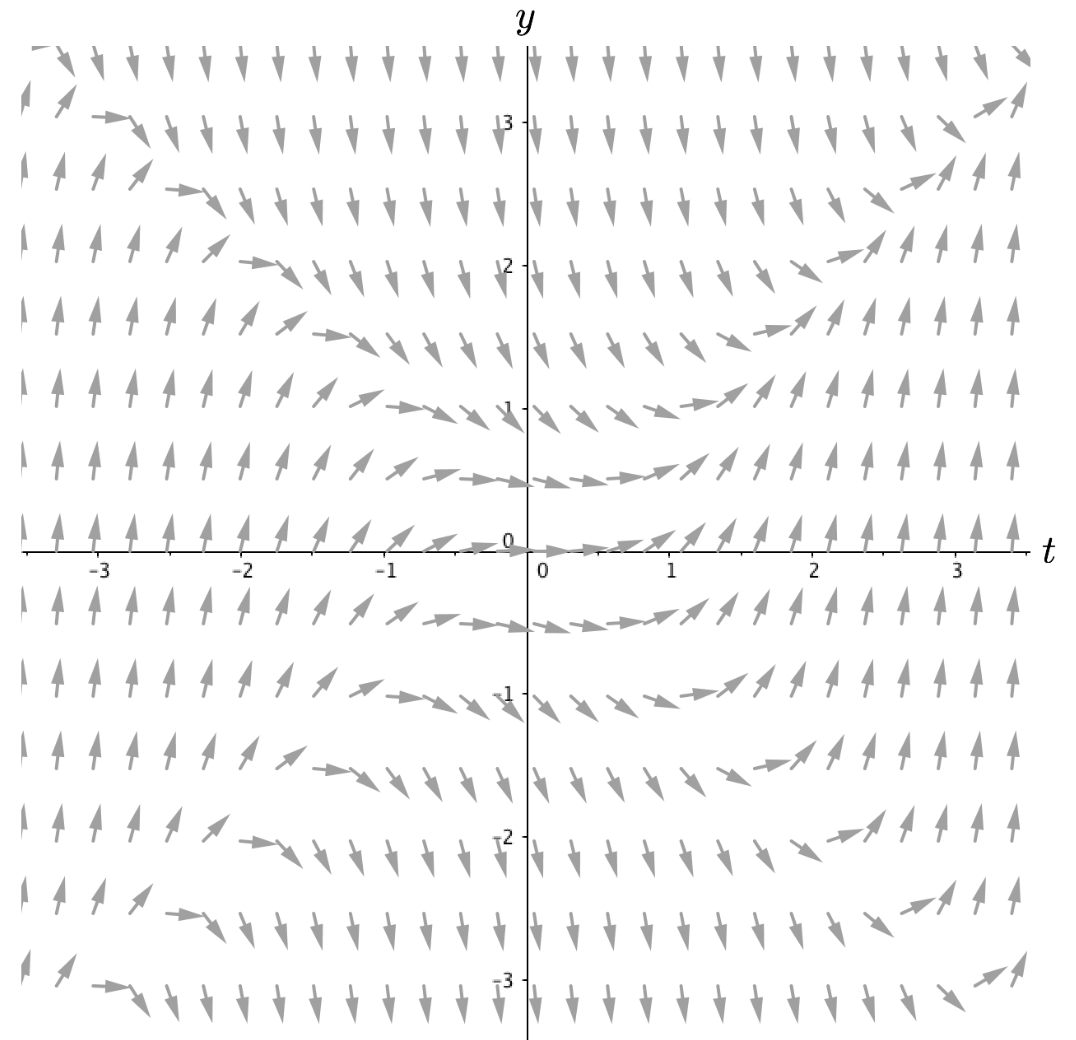
\includegraphics[width=2.75in]{02/02SlopeField2.png} \label{01problem8partb}
\end{enumerate*}

\begin{enumerate*}[resume]
\item 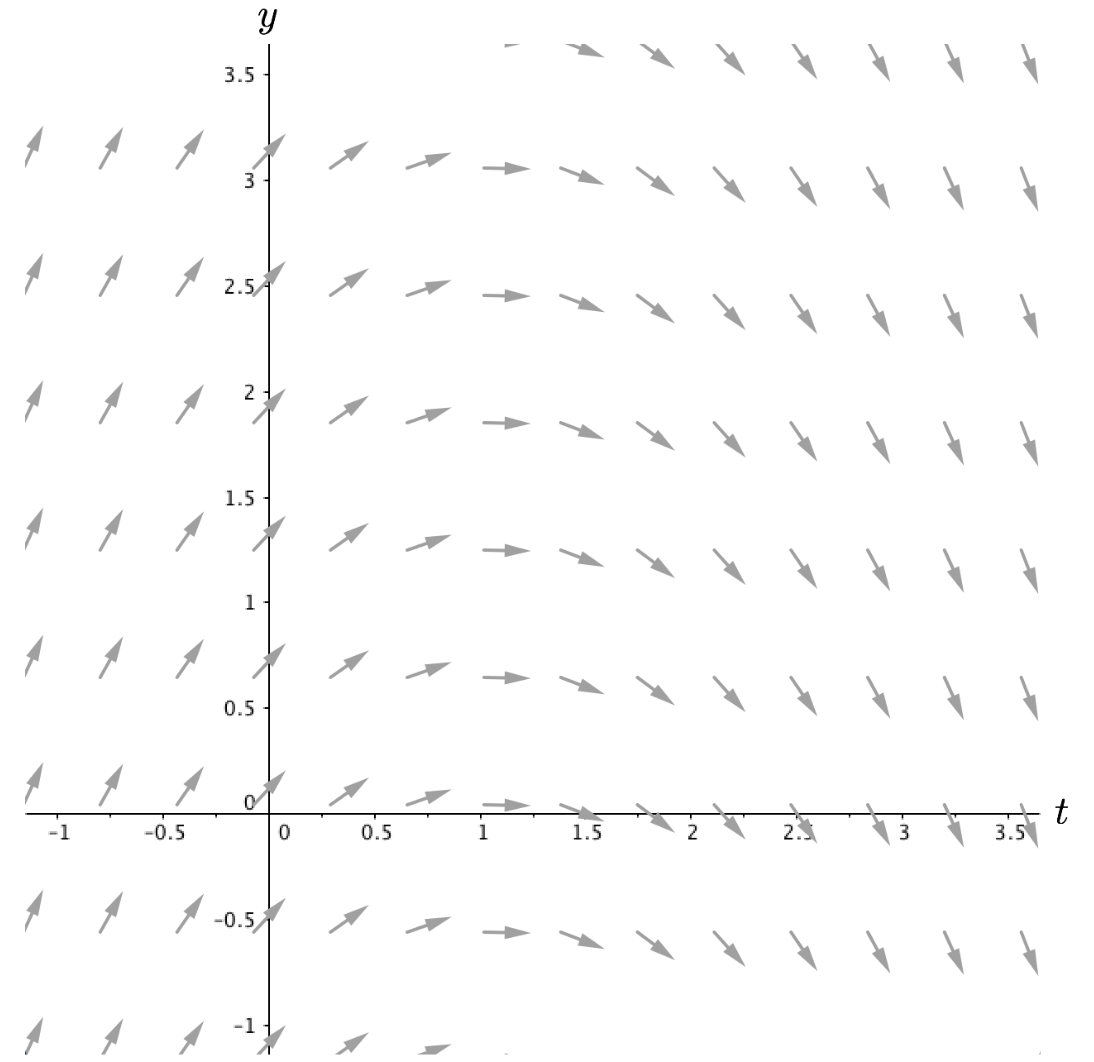
\includegraphics[width=2.75in]{02/02SlopeField3.png} \label{01problem8partc}
\end{enumerate*}
\vspace{0.1in}
\item For each of the slope fields in the previous problem, sketch in graphs of several different qualitatively correct solutions. \label{01problem9}
\vfill

\end{enumerate}


